\section{Systém iterovaných funkcí}\label{sec:ifs}

V předchozí části kapitoly viděli, jak lze fraktální objekty efektivně popisovat pomocí L-systémů, kde struktura vzniká paralelním přepisováním symbolů a jejich vizualizace se provádí prostřednictvím želví grafiky. Tento přístup nám umožňoval popsat určitou skupinu fraktálů, nicméně pro jiné fraktály by se nám hodil vhodnější popis jejich konstrukce. Např. Sierpińského trojúhelník lze popsat pomocí L-systému, nicméně v sekci \ref{sec:sobepodobnost} o soběpodobnosti jsme si jej záváděli spíše pomocí opakované aplikace určitých geometrických transformací (ač jsme neuvedli jejich explicitní vyjádření). Ty si později zavedeme jako tzv. \emph{systémy iterovaných funkcí}\index{systém iterovaných funkcí}.

Nejdříve se podíváme trochu více na matematickou podstatu. Hodně záležitostí jsme si již rozebrali v kapitole \ref{chapter:hausdorffuv-mp} o Hausdorffově metrickém prostoru\index{Hausdorffův metrický prostor}\index{metrický prostor!Hausdorffův}, který zde bude hrát významnou roli, a dále na ně budeme navazovat. Pro související matematickou teorii, kterou zde dále budeme vykládat, doporučuji knihu \cite{Barnsley1993}.

\subsection{Kontrakce na Hausdorffově metrickém prostoru}\label{subsec:hausdorffuv-mp-kontrakce}

V minulých kapitolách jsme se často zaměřovali na lipschitzovská a bilipschitzovská zobrazení. V tomto případě nás budou speciálně zajímat tzv. \emph{kontrakce}\index{kontrakce}\index{zobrazení!kontraktivní}. Těmto termínům a faktům s nimi souvisejícími jsme se krátce věnovali v podsekci \ref{subsec:lipschitzovska-zobrazeni}.

Připomeňme, že lipschitzovské zobrazení rovnou implikuje spojist v libovolném metrickém prostoru $(X,\varrho)$. Ještě však než začneme, podíváme se na alternativní definici Hausdorffovy metriky, která se nám dále bude hodit.
\begin{theorem}[Alternativní definice Hausdorffovy metriky]\label{thm:alternativni-hausdorffova-metrika}
    Nechť $(X,\varrho)$ je metrický prostor. Pro každé $A,B\in\hyperspace(X)$ platí
    \[\hausdorffmetric(A,B)=\max\set{\sup_{x\in A}\varrho(x,B),\sup_{y\in B}\varrho(y,A)}.\]
\end{theorem}
\begin{proof}
    Nechť je dáno $\varepsilon>0$, takové, že $\varepsilon\geqslant\hausdorffmetric(A,B)$. Pak $A\subseteq(B)_\varepsilon$ a $B\subseteq(A)_\delta$, tzn.
    \[\varepsilon\geqslant\max\set{\sup_{x\in A}\varrho(x,B),\sup_{y\in B}\varrho(y,A)}.\]
    Naopak zvolíme-li $0<\varepsilon\leqslant\hausdorffmetric(A,B)$, pak určitě platí alespoň jedna z nerovností:
    \[\varepsilon\leqslant\sup_{x\in A}\varrho(x,B)\;\text{nebo}\;\varepsilon\leqslant\sup_{y\in B}\varrho(y,A).\]
    Tedy
    \[\varepsilon\leqslant\max\set{\sup_{x\in A}\varrho(x,B),\sup_{y\in B}\varrho(y,A)}.\]
    Z toho dostáváme závěr tvrzení.
\end{proof}

Jako první se podíváme na trojici pomocných lemmat.
\begin{lemma}\label{lem:spojitost-a-hyperprostor}
    Nechť $\mapping{f}{X}{X}$ je spojisté zobrazení v metrickém prostoru $(X,\varrho)$. Pak pro každé $S\in\hyperspace(X)$ platí $f(S)\in\hyperspace(X)$.
\end{lemma}
\begin{proof}
    Nechť $S\in\hyperspace(X)$. Zjevně platí $f(S)\neq\emptyset$. Pro důkaz kompaktnosti $f(S)$ uvažujme posloupnost $\set{x_n}_{n=1}^\infty$, kde $x_i\in S$ pro každé $i\in\N$. Protože $S$ je kompaktní, existuje posloupnost indexů $\set{n_k}_{k=1}^\infty$, taková, že $x_{n_k}\to x\in S$. Ze spojitosti zobrazení $f$ však plyne, že pak $\set{f(x_{n_k})}_{k=1}^\infty$ je podposloupností posloupnosti $\set{f(x_n)}_{n=1}^\infty$ a $f(x_{n_k})\to f(x)$, tedy i $f(S)$ je kompaktní.
\end{proof}
\begin{lemma}\label{lem:kontrakce-a-hyperprostor}
    Nechť $\mapping{f}{X}{X}$ je kontrakce na metrickém prostoru $(X,\varrho)$ s faktorem $0<K<1$. Pak $\mapping{f}{\hyperspace(X)}{\hyperspace(X)}$ je kontrakce na Hausdorffově metrickém prostoru s faktorem $K$.
\end{lemma}
(Převzato z \citep[str. 79]{Barnsley1993}.)
\begin{proof}
    Z předchozího lemmatu \ref{lem:spojitost-a-hyperprostor} víme, že $f(S)\in\hyperspace(X)$ pro každé $S\in\hyperspace(X)$. Mějme množiny $A,B\in\hyperspace(X)$. Pak
    \begin{align*}
        \varrho(f(A),f(B))&=\inf\set{\varrho(f(x),f(y))\mid x\in A\;,\;y\in B}\\
        &\leqslant\inf\set{K\cdot\varrho(x,y)\mid x\in A\;,\;y\in B}\\
        &=K\cdot\inf\set{\varrho(x,y)\mid x\in A\;,\;y\in B}\\
        &=K\cdot\varrho(A,B).
    \end{align*}
    Tedy celkově
    \begin{align*}
        \hausdorffmetric(f(A),f(B))&=\inf\set{\delta>0\mid f(A)\subseteq(f(B))_\delta\land f(B)\subseteq(f(A))_\delta}\\
        &=\max\set{\sup_{x\in A}\varrho(f(x),f(B)),\sup_{y\in B}\varrho(f(y),f(A))}\\
        &=\max\set{\sup_{x\in A}\inf_{y\in B}\varrho(f(x),f(y)),\sup_{y\in B}\inf_{x\in A}\varrho(f(y),f(x))}\\
        &\leqslant K\max\set{\sup_{x\in A}\inf_{y\in B}\varrho(f(x),f(y)),\sup_{y\in B}\inf_{x\in A}\varrho(f(y),f(x))}\\
        &=K\hausdorffmetric(A,B).
    \end{align*}
    Druhá rovnost plyne z věty \ref{thm:alternativni-hausdorffova-metrika}.
\end{proof}
(Převzato a upraveno z \citep[str. 79]{Barnsley1993}.)
\begin{lemma}\label{lem:hausdorffova-metrika-odhad-sjednoceni}
    Pro každé $A,B,C,D\in\hyperspace(X)$, kde $(X,\varrho)$ je metrický prostor, platí
    \[\hausdorffmetric(A\cup B,C\cup D)\leqslant\max\set{\hausdorffmetric(A,C),\hausdorffmetric(B,D)}.\]
\end{lemma}
\begin{proof}
    Budeme vycházet z alternativní definice Hausdorffovy metriky (viz věta \ref{thm:alternativni-hausdorffova-metrika}). Pro $\varrho(x,A\cup B)$ platí následující odhad:
    \[\varrho(x,A\cup B)=\min\set{\inf_{y\in A}\varrho(x,y),\inf_{z\in B}\varrho(x,z)}\leqslant\inf_{y\in A}\varrho(x,y)=\varrho(x,A).\]
    Z toho pak máme
    \[\sup_{x\in A}\varrho(x,C\cup D)\leqslant\sup_{x\in A}\inf_{y\in C}\varrho(x,y)=\varrho(x,A)\leqslant\hausdorffmetric(A,C)\]
    a tedy
    \[\sup_{x\in A\cup B}\varrho(x,C\cup D)\leqslant\max\set{\hausdorffmetric(A,C),\hausdorffmetric(B,D)}.\]
    Stejný odhad lze získat i pro $\sup_{x\in C\cup D}\varrho(x,A\cup B)$:
    \begin{align*}
        \sup_{x\in C\cup D}\varrho(x,A\cup B)&=\max\set{\sup_{x\in C}\varrho(x,A\cup B),\sup_{x\in D}\varrho(x,A\cup B)}\\
        &\leqslant\max\set{\hausdorffmetric(C,A),\hausdorffmetric(D,B)}=\max\set{\hausdorffmetric(A,C),\hausdorffmetric(B,D)}.
    \end{align*}
    Tedy celkově lze psát
    \begin{align*}
        \hausdorffmetric(A\cup B,C\cup D)&=\max\set{\sup_{x\in A\cup B}\varrho(x,C\cup D),\sup_{x\in C\cup D}\varrho(x,A\cup B)}\\
        &\leqslant\max\set{\hausdorffmetric(A,C),\hausdorffmetric(B,D)}.
    \end{align*}
\end{proof}

Dvojice lemmat \ref{lem:spojitost-a-hyperprostor} a \ref{lem:kontrakce-a-hyperprostor} nám v podstatě říká, že obrazem kompaktní množiny v kontraktivním zobrazení\index{zobrazení!kontraktivní}\index{kontraktivní zobrazení} je opět kompaktní množina a že "kontraktivita" zobrazení definovaného na libovolném metrickém prostoru $(X,\varrho)$ se zachovává na hyperprostoru. Tento výsledek se nám bude později hodit, neboť neboť jak již bylo zmíněno na začátku, některé fraktály lze konstruovat pomocí opakované aplikace určitých geometrických tranformací. Jak lze nejspíše z dosavadního výkladu tušit, budeme pracovat právě s kontrakcemi.
\begin{definition}[Systém iterovaných funkcí]\label{def:system-iterovanych-funkci}
    \emph{Systém iterovaných funkcí}\index{systém iterovaných funkcí}, zkráceně IFS (z anglického \emph{iterated function system}\index{iterated function system}), na metrickém prostoru $(X,\varrho)$ je konečná množina kontrakcí
    \[\set{\mapping{\psi_i}{X}{X}\mid 1\leqslant i\leqslant n}\]
    s faktory $K_i$. Kontraktivním faktorem IFS je číslo $K=\max\set{K_i\mid 1\leqslant i\leqslant n}$.
\end{definition}
Zatím není zcela zjevné, proč definujeme pro IFS kontraktivní faktor jako maximum z faktorů všech kontrakcí v něm obsažených (byť to může působit do jisté míry intuitivně). Odpověď na tuto otázku nám poskytne následující věta \ref{thm:sjednoceni-kontrakci}.
\begin{theorem}\label{thm:sjednoceni-kontrakci}
    Nechť $\set{\psi_1,\psi_2,\ldots,\psi_n}$ je IFS na metrickém prostoru $(X,\varrho)$ s kontraktivním faktorem\index{faktor}\index{kontraktivní faktor}\index{faktor!kontraktivní} $0<K<1$. Pak zobrazení $\mapping{\Psi}{\hyperspace(X)}{\hyperspace(X)}$ definované předpisem
    \[\Psi(A)=\bigcup_{i=1}^n\psi_i(A)\]
    pro $A\in\hyperspace(X)$ je kontrakce na $(\hyperspace(X),\hausdorffmetric)$ s faktorem $K$.
\end{theorem}
(Převzato z \citep[str. 81]{Barnsley1993}.)
\begin{proof}
    Důkaz tvrzení lze provést indukcí podle $n$. V případě, kdy $n=1$ je situace triviální. Pro $n=2$ zvolme množiny $A,B\in\hyperspace(X)$. Pak
    \begin{align*}
        \hausdorffmetric(\psi_1(A)\cup\psi_2(A),\psi_1(B)\cup\psi_2(B))&\leqslant\max\set{\hausdorffmetric(\psi_1(A),\psi_1(B)),\hausdorffmetric(\psi_2(A),\psi_2(B))}\\
        &\leqslant\max\set{K_1\hausdorffmetric(A,B),K_2\hausdorffmetric(A,B)}\\
        &\leqslant K\hausdorffmetric(A,B),
    \end{align*}
    kde druhá nerovnost plyne z lemmatu \ref{lem:hausdorffova-metrika-odhad-sjednoceni}. Nyní ukážeme, že zobrazení $\Psi
    $ definované předpisem $\Psi(A)=\bigcup_{i=1}^n\psi_i(A)$ je kontrakce. Mějme opět množiny $A,B\in\hyperspace(X)$. Pak
    \begin{align*}
        \hausdorffmetric(\Psi(A),\Psi(B))&=\hausdorffmetric\left(\left(\bigcup_{i=1}^{n-1}\psi_i(A)\right)\cup\psi_n(A),\left(\bigcup_{i=1}^{n-1}\psi_i(B)\right)\cup\psi_n(B)\right)\\
        &\leqslant\max\set{\hausdorffmetric\left(\bigcup_{i=1}^{n-1}\psi_i(A),\bigcup_{i=1}^{n-1}\psi_i(B)\right),\hausdorffmetric(\psi_n(A)\cup\psi_n(B))}\\
        &\stackrel{\text{I.P.}}{\leqslant}\max\set{K\hausdorffmetric(A,B),K_n\hausdorffmetric(A,B)}\leqslant K\hausdorffmetric(A,B).
    \end{align*}
\end{proof}
\begin{remark}
    Dodejme, že dále v textu budeme používat značení $\Psi^{\circ n}$ definované induktivně:
    \begin{align*}
        \Psi^{\circ 0}=\id,\\
        \Psi^{\circ n}=\Psi\circ\Psi^{\circ(n-1)}\;,\;n\in\N.
    \end{align*}
    Tzn. pro libovolnou množinu $B\in\hyperspace(X)$ je
    \[\Psi^{\circ 0}(B)=B\;\text{a}\;\Psi^{\circ n}(B)=\Psi(\Psi^{\circ(n-1)}(B)).\]
\end{remark}

S kontrakcemi se pojí známá věta z matematické analýzy, která se nazývá \emph{Banachova věta o pevném bodě} (vit \ref{thm:banach}).
\begin{definition}[Pevný bod]\label{def:pevny-bod}
    Bod $x\in X$ se nazývá pevným bodem zobrazení $\mapping{f}{X}{X}$, pokud $f(x)=x$.
\end{definition}
\begin{theorem}[Banachova věta o pevném bodě]\label{thm:banach}
    Nechť $(X,\varrho)$ je úplný metrický prostor a zobrazení $\mapping{f}{X}{X}$ je kontrakce. Pak existuje právě jeden pevný bod $x\in X$ zobrazení $f$. Navíc volíme-li $x_0\in\N$ libovolně a $x_n=f(x_{n-1})$ pro každé $n\in\N$, pak $x_n\to x$.
\end{theorem}
\begin{proof}
    Podle předpokladu je $f$ kontrakce s faktorem $K$. Zvolme $x_0\in X$ a dále pro každé $n\in\N$ položme $x_n=f(x_{n-1})$. Ukážeme, že takto definovaná posloupnost budů má limitu. Podle předpokladu je $(X,\varrho)$ úplný metrický prostor, tedy stačí ukázat, že posloupnost $\set{x_n}_{n=1}^\infty$ je cauchyovská. Pro vzdálenosti dvou po sobě jdoucích členů platí
    \begin{align*}
        \varrho(x_1,x_2)&=\varrho(f(x_0),f(x_1))\leqslant K\varrho(x_0,x_1),\\
        \varrho(x_2,x_3)&=\varrho(f(x_1),f(x_2))\leqslant K\varrho(x_1,x_2)\leqslant K^2\varrho(x_0,x_1),\\
        \varrho(x_3,x_4)&=\varrho(f(x_2),f(x_3))\leqslant K\varrho(x_2,x_3)\leqslant K^3\varrho(x_0,x_1),\\
        &\vdots\\
        \varrho(x_i,x_{i+1})&=\varrho(f(x_{i-1}),f(x_i))\leqslant K\varrho(x_{i-1},x_i)\leqslant K^i\varrho(x_0,x_1).\\
        &\vdots
    \end{align*}
    Pro odhadnutí vzdálenosti dvojice členů, které nejdou nutně bezprostředně po sobě použijeme trojúhelníkovou nerovnost. Volme $n,m\in\N$, pričemž $m>n$. Pak lze psát
    \begin{align*}
        \varrho(x_n,x_m)&\leqslant\sum_{i=n}^{m-1}\varrho(x_i,x_{i+1})\leqslant\sum_{i=n}^{m-1}K^i\varrho(x_0,x_1)=K^n\varrho(x_0,x_1)\sum_{i=1}^{m-n-1}K^i\\
        &=K^n\varrho(x_0,x_1)\cdot\dfrac{1-K^{n-m}}{K-1}.
    \end{align*}
    Výraz na pravé straně má pro $n\to\infty$ limitu $0$, tedy posloupnost $\set{x_n}_{n=1}^\infty$ je cauchyovská a má limitu $x\in X$. Dále ze spojitosti funkce $f$ (neboť je lipschitzovská) plyne
    \[x=\lim_{n\to\infty}x_{n+1}=\lim_{n\to\infty}f(x_n)=f(x),\]
    tedy $x\in X$ je pevným bodem $f$. Jednoznačnost pevného bodu $x$ lze ukázat sporem. Pokud by existoval další pevný bod $y\neq x$, pak
    \[\varrho(x,y)=\varrho(f(x),f(y))\leqslant K\varrho(x,y).\]
    Protože $\varrho(x,y)>0$, musí být $K\geqslant 1$, což je spor s předpokladem, že $f$ je kontrakce.
\end{proof}
Speciálně pro zobrazení $\Psi$ definované ve větě \ref{thm:sjednoceni-kontrakci} nám Banachova věta \ref{thm:banach} nejen říká, že má právě jeden pevný bod $A\in\hyperspace(X)$, tzn. $\Psi(A)=A$, ale zároveň udává způsob, jak daný pevný bod nalézt. Stačí opakovaně iterovat dané zobrazení.
\begin{definition}[Atraktor]\label{def:atraktor}
    Pevný bod $A\in\hyperspace(X)$ zobrazení $\Psi$ definovaného ve větě \ref{thm:sjednoceni-kontrakci} pro libovolné IFS se nazývá \emph{atraktor}\index{atraktor}.
\end{definition}
Z Banachovy věty speciálně plyne, že atraktor $A$ libovolného IFS lze určit jako následující limitu:
\[A=\lim_{n\to\infty}\Psi^{\circ n}(B),\]
kde $B\in\hyperspace(X)$. Zajímavostí je fakt, že výsledný atraktor $A$ je zcela nezávislý na volbě množiny $B$. Tento fakt si ještě přiblížíme v podsekci \ref{subsec:fraktaly-ifs}.

V dalším textu budeme pracovat především s afinními zobrazeními v $\R^n$ se standardní eukleidovskou metrikou. Připomeňme si zde, že afinním zobrazením rozumíme jakékoliv zobrazení $\mapping{f}{X}{X}$, takové, že
\[f(x)=\mat{A}x+b,\]
kde $b\in X$ a $\mat{A}$ je regulární matice. O afinnitách lze též dokázat řadu zajímavých tvrzení, avšak tyto záležitosti již spadají spíše do oblasti lineární algebry. Avšak v případě každé z afinnit, které zde dále uvidíme, se čtenář může celkem snadno přesvědčit, že se skutečně jedná o kontrakci.

\subsection{Frakrály generované pomocí IFS}\label{subsec:fraktaly-ifs}

V předešlé podsekci \ref{subsec:hausdorffuv-mp-kontrakce} jsme se společně podívali na některé důležité poznatky týkající se kontrakcí a Hausdorffova metrického prostoru (viz kapitola \ref{chapter:hausdorffuv-mp}). Na některá dokázaná tvrzení se zde budeme odkazovat.

Protože pracujeme s fraktálními útvary v rovině, tj. $\R^2$, afinní zobrazení, s nimiž budeme pracovat, budou mít tvar
\begin{equation}\label{eq:afinita-v-R2}
    \psi\left(\begin{matrix}
        x\\
        y
    \end{matrix}\right)=\underbrace{\left(\begin{matrix}
        a & b\\
        c & d
    \end{matrix}\right)}_{\mat{A}}\left(\begin{matrix}
        x\\
        y
    \end{matrix}\right)+\left(\begin{matrix}
        e\\
        f
    \end{matrix}\right).
\end{equation}
Připomeňme, že matice $\mat{A}$ je regulární. Podíváme se na některé fraktály, které jsme již viděli v úvodní kapitole \ref{chapter:uvod_do_fraktalu} v sekci \ref{sec:sobepodobnost}. Jiný způsob generování těchto a mnohých jiných fraktálních útvarů nám poskytují L-systémy, které jsme si ilustrovali v sekci \ref{sec:L-systemy}.

Znovu se podívejme na asi jeden z nejznáměnších fraktálů z této kategorie -- Sierpińského trojúhelník. Jeho konstrukce lze docílit pomocí IFS $\set{\omega_1,\omega_2,\omega_3}$, přičemž $\mapping{\omega_1,\omega_2,\omega_3}{\R^2}{\R^2}$ a jednotlivé kontrakce jsou definovány následujícími předpisy:
\begin{align*}
    \omega_1\left(\begin{matrix}
        x\\
        y
    \end{matrix}\right)&=\left(\begin{matrix}
        1/2 & 0\\
        0 & 1/2
    \end{matrix}\right)\left(\begin{matrix}
        x\\
        y
    \end{matrix}\right)+\left(\begin{matrix}
        0\\
        0
    \end{matrix}\right),\\
    \omega_2\left(\begin{matrix}
        x\\
        y
    \end{matrix}\right)&=\left(\begin{matrix}
        1/2 & 0\\
        0 & 1/2
    \end{matrix}\right)\left(\begin{matrix}
        x\\
        y
    \end{matrix}\right)+\left(\begin{matrix}
        1/2\\
        0
    \end{matrix}\right),\\
    \omega_3\left(\begin{matrix}
        x\\
        y
    \end{matrix}\right)&=\left(\begin{matrix}
        1/2 & 0\\
        0 & 1/2
    \end{matrix}\right)\left(\begin{matrix}
        x\\
        y
    \end{matrix}\right)+\left(\begin{matrix}
        1/4\\
        \sqrt{3}/4
    \end{matrix}\right).
\end{align*}
Tedy zobrazení $\mapping{\Omega}{\hyperspace(\R^2)}{\hyperspace(\R^2)}$ definujeme jako
\[\Omega(A)=\omega_1(A)\cup\omega_2(A)\cup\omega_3(A),\]
kde $A\in\hyperspace(\R^2)$. Připomeňme, že takto definované $\Omega^n$ je kontrakce (podle věty \ref{thm:sjednoceni-kontrakci}) a tedy z Banachovy věty o pevném bodě plyne (viz věta \ref{thm:banach}), že má právě jeden atraktor, tj. množina $A\in\hyperspace(\R^2)$, že platí $A=\Omega(A)$. Kontraktivní faktor tohoto (ani jiného) IFS nás vyloženě zajímat nemusí, avšak není těžké jej dopočítat. Např. zde je celkem zjevné, že $K=1/2$. Užitečnější je však pro nás fakt, že atraktor $A$ lze určit jako
\[A=\lim_{n\to\infty}\Omega^{\circ n}(B),\]
kde $B\in\hyperspace(\R^2)$. V našem případě je počítečním útvarem rovnostranný trojúhelník $T$, jehož vrcholy mají souřadnice
\[\left(\begin{matrix}
    0\\
    0
\end{matrix}\right),\;\left(\begin{matrix}
    1\\
    0
\end{matrix}\right),\;\left(\begin{matrix}
    1/2\\
    \sqrt{3}/2
\end{matrix}\right).\]
Prvních několik iterací zobrazení $\Omega$ si lze prohlédnout na obrázku \ref{fig:iterace-zobrazeni-omega-sierpinskeho-trojuhelnik}. Sierpińského trojúhelník je tedy atraktorem zobrazení $\Omega$.
\begin{figure}[h]
    \centering
    \begin{subfigure}{0.45\textwidth}
        \centering
        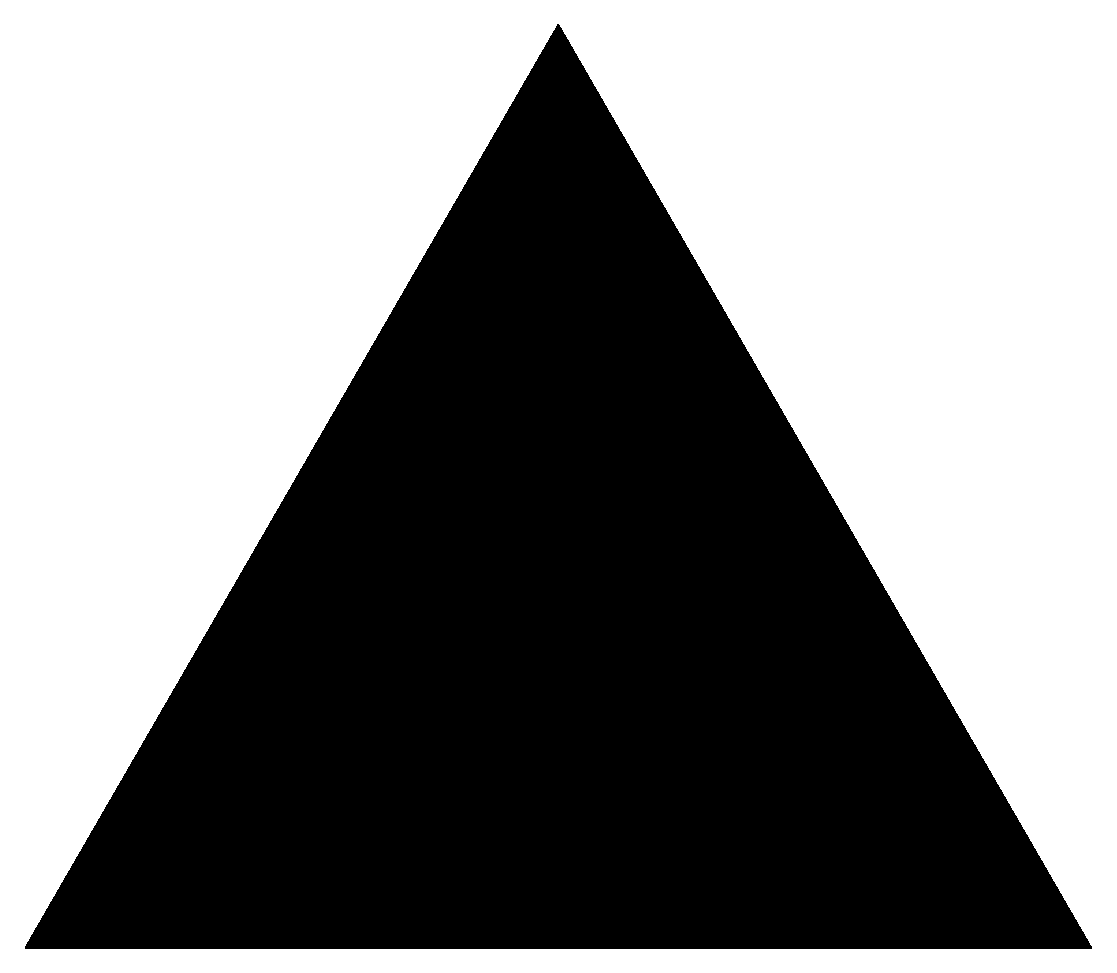
\includegraphics[width=\textwidth]{sierpinsky-triangle-iter0.pdf}
        \begin{center}
            $n=0$
        \end{center}
    \end{subfigure}
    \qquad
    \vspace{1cm}
    \begin{subfigure}{0.45\textwidth}
        \centering
        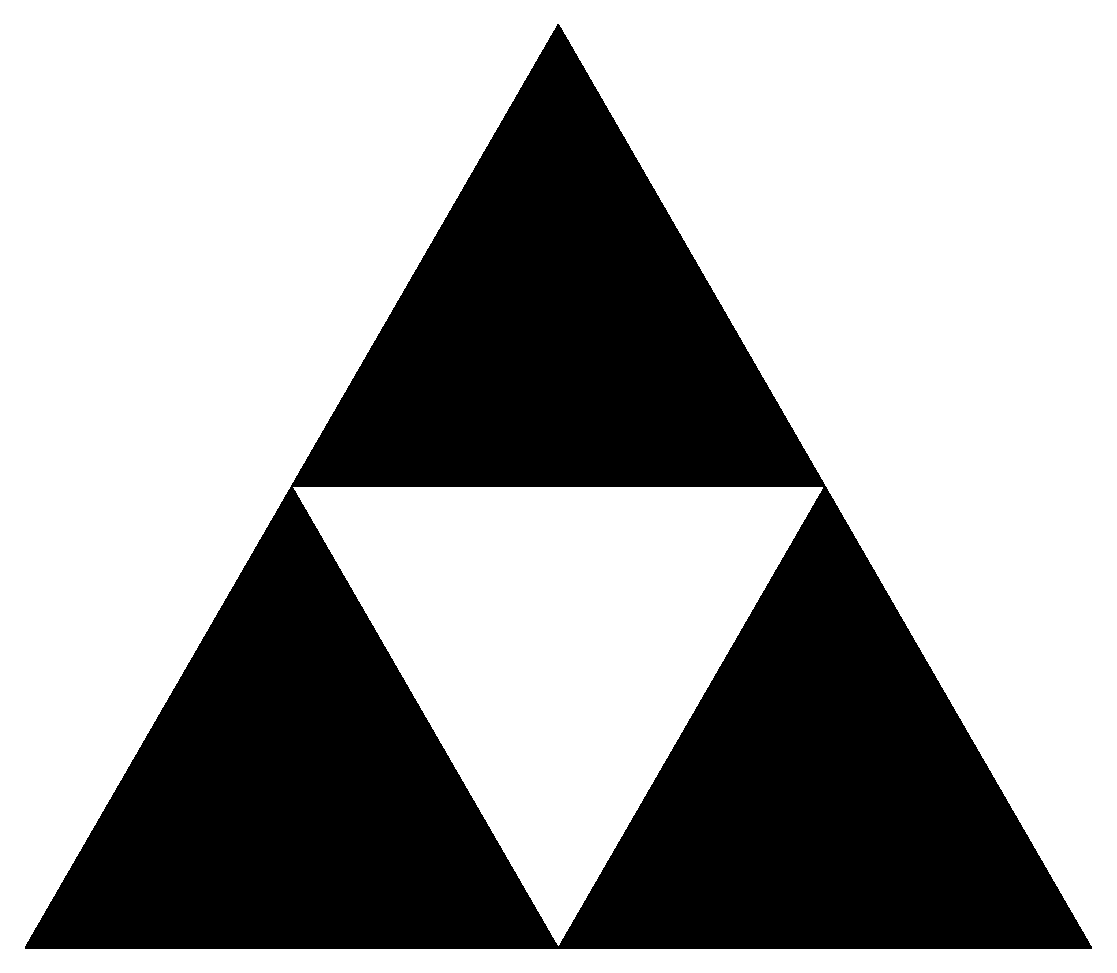
\includegraphics[width=\textwidth]{sierpinsky-triangle-iter1.pdf}
        \begin{center}
            $n=1$
        \end{center}
    \end{subfigure}
    \qquad
    \begin{subfigure}{0.45\textwidth}
        \centering
        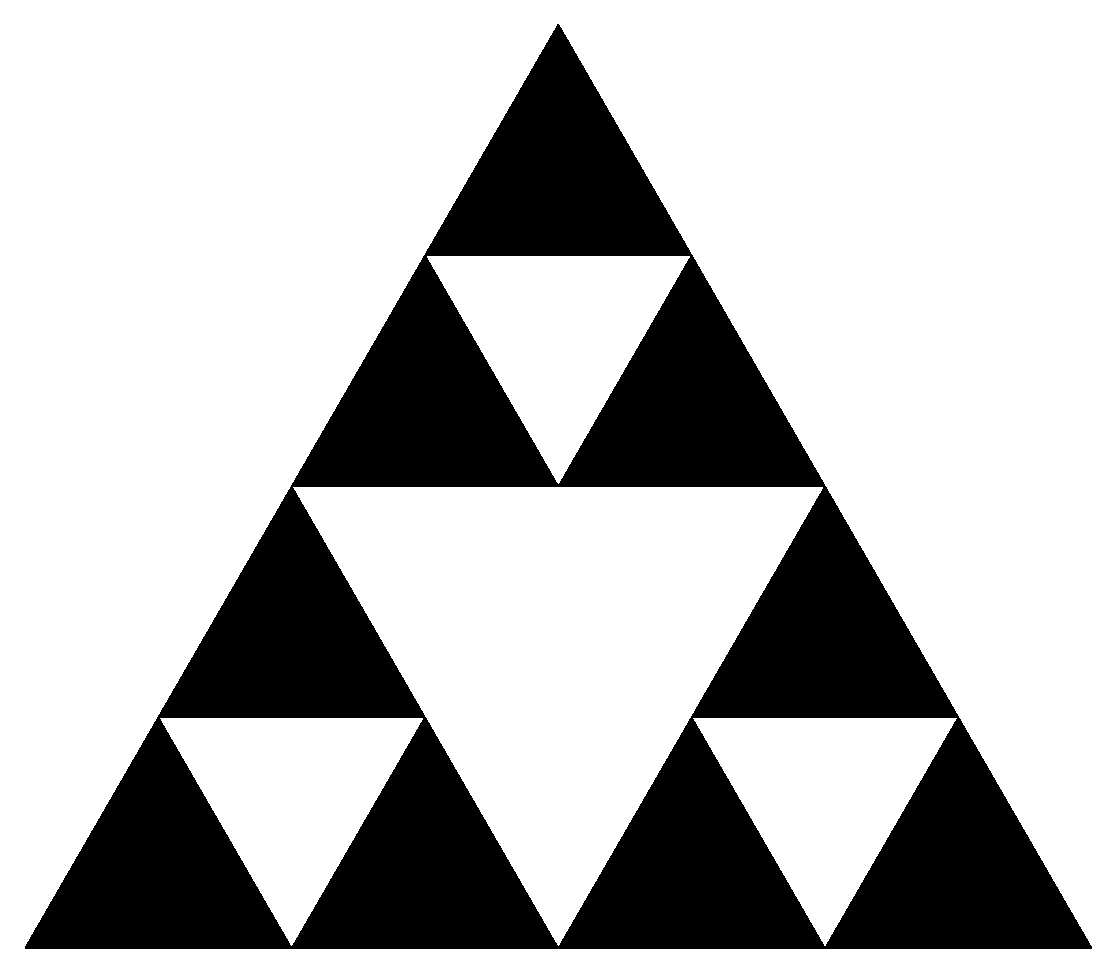
\includegraphics[width=\textwidth]{sierpinsky-triangle-iter2.pdf}
        \begin{center}
            $n=2$
        \end{center}
    \end{subfigure}
    \qquad
    \vspace{1cm}
    \begin{subfigure}{0.45\textwidth}
        \centering
        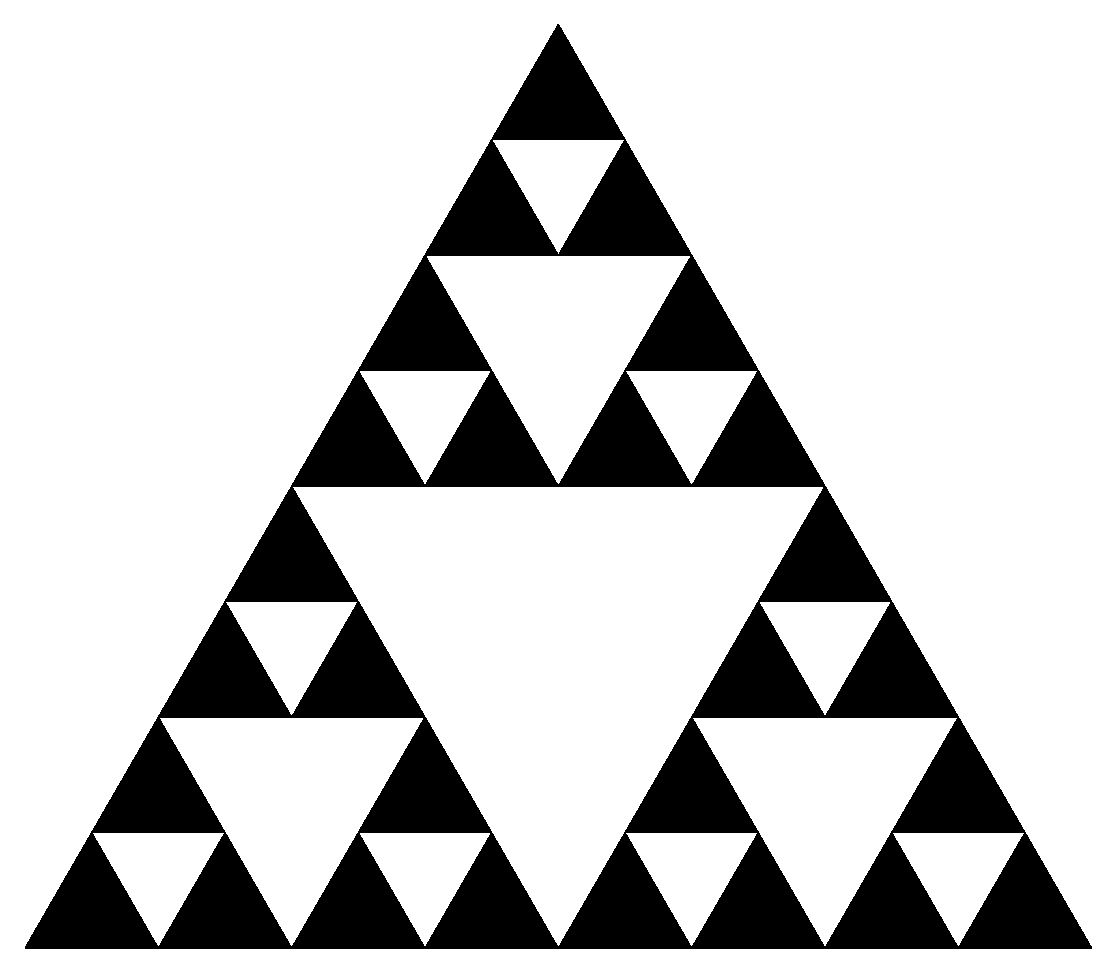
\includegraphics[width=\textwidth]{sierpinsky-triangle-iter3.pdf}
        \begin{center}
            $n=3$
        \end{center}
    \end{subfigure}
    \qquad
    \begin{subfigure}{0.45\textwidth}
        \centering
        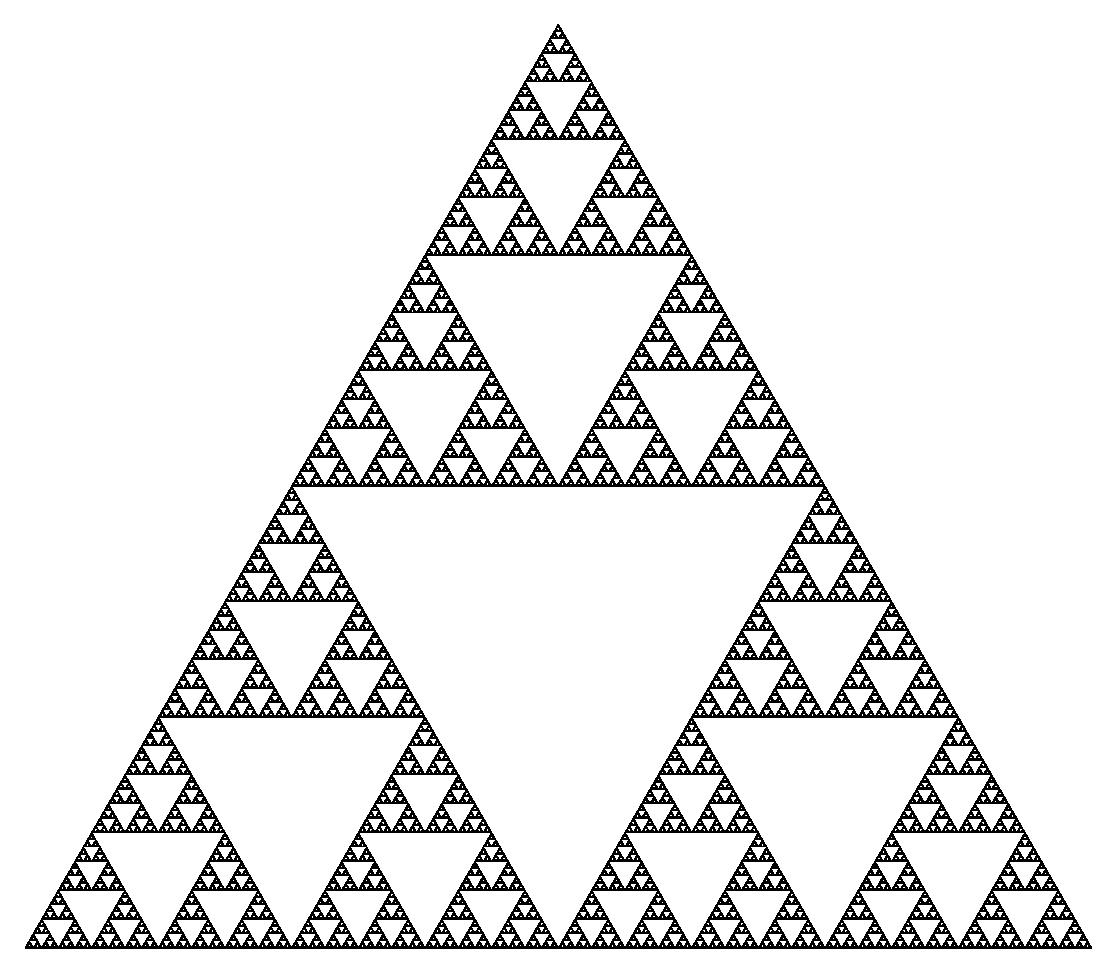
\includegraphics[width=\textwidth]{sierpinsky-triangle-iter8.pdf}
        \begin{center}
            $n=8$
        \end{center}
    \end{subfigure}
    \caption{Iterace zobrazení $\Omega$}
    \label{fig:iterace-zobrazeni-omega-sierpinskeho-trojuhelnik}
\end{figure}
Zajímavostí je, že atraktor daného IFS je zcela nezávislý na volbě počátečního útvaru. Ač je tedy běžné, že v případě Sierpińského trojúhelníka začínáme s rovnostranným trojúhelníkem, faktem je, že je zcela lhostejné\footnote{Z formálního hlediska je třeba, aby se jednalo o kompaktní neprázdnou množinu, nicméně v $\R^n$ stačí pro tento účel uvažovat všechny neprázdné množiny, které \emph{uzavřené a omezené} (viz věta \ref{thm:heine-borel})}, se kterým útvarem začneme (viz obrázek \ref{fig:iterace-zobrazeni-omega-sierpinskeho-trojuhelnik-jiny-poc-utvar}).
\begin{figure}[h]
    \centering
    \begin{subfigure}{0.45\textwidth}
        \centering
        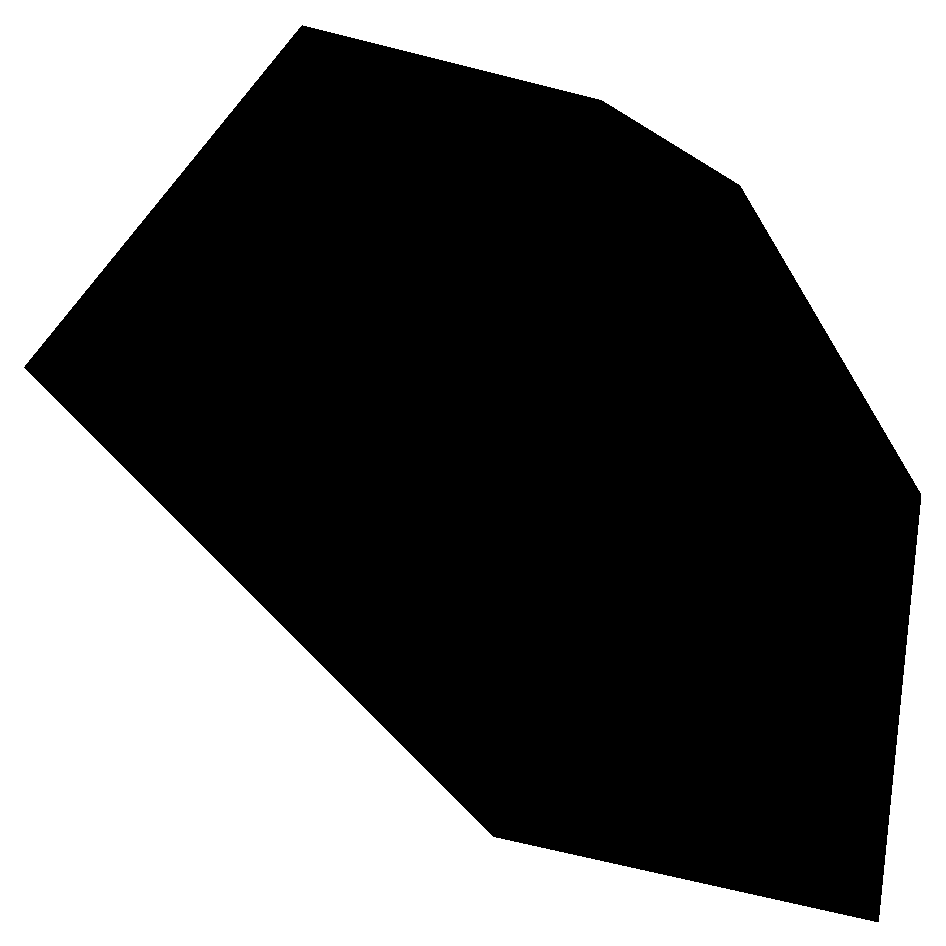
\includegraphics[width=\textwidth]{sierpinsky-triangle-2-iter0.pdf}
        \begin{center}
            $n=0$
        \end{center}
    \end{subfigure}
    \qquad
    \vspace{1cm}
    \begin{subfigure}{0.45\textwidth}
        \centering
        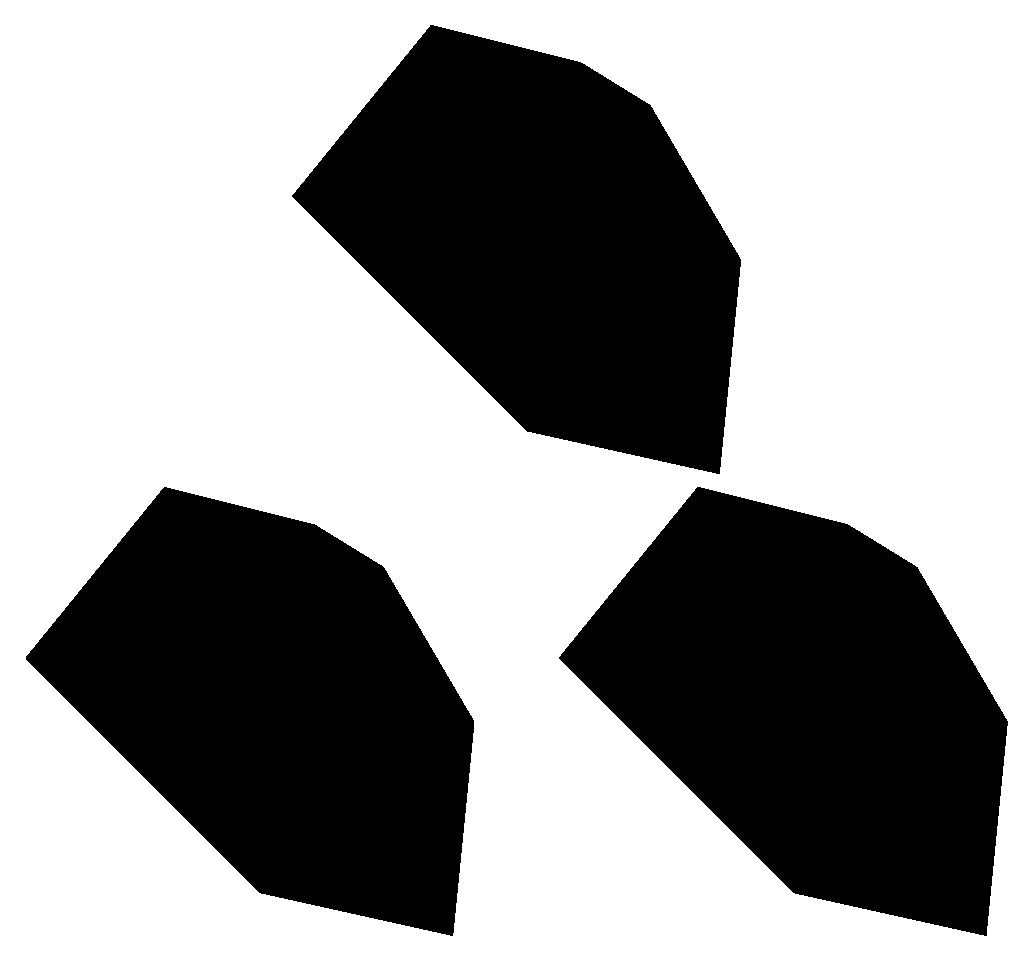
\includegraphics[width=\textwidth]{sierpinsky-triangle-2-iter1.pdf}
        \begin{center}
            $n=1$
        \end{center}
    \end{subfigure}
    \qquad
    \begin{subfigure}{0.45\textwidth}
        \centering
        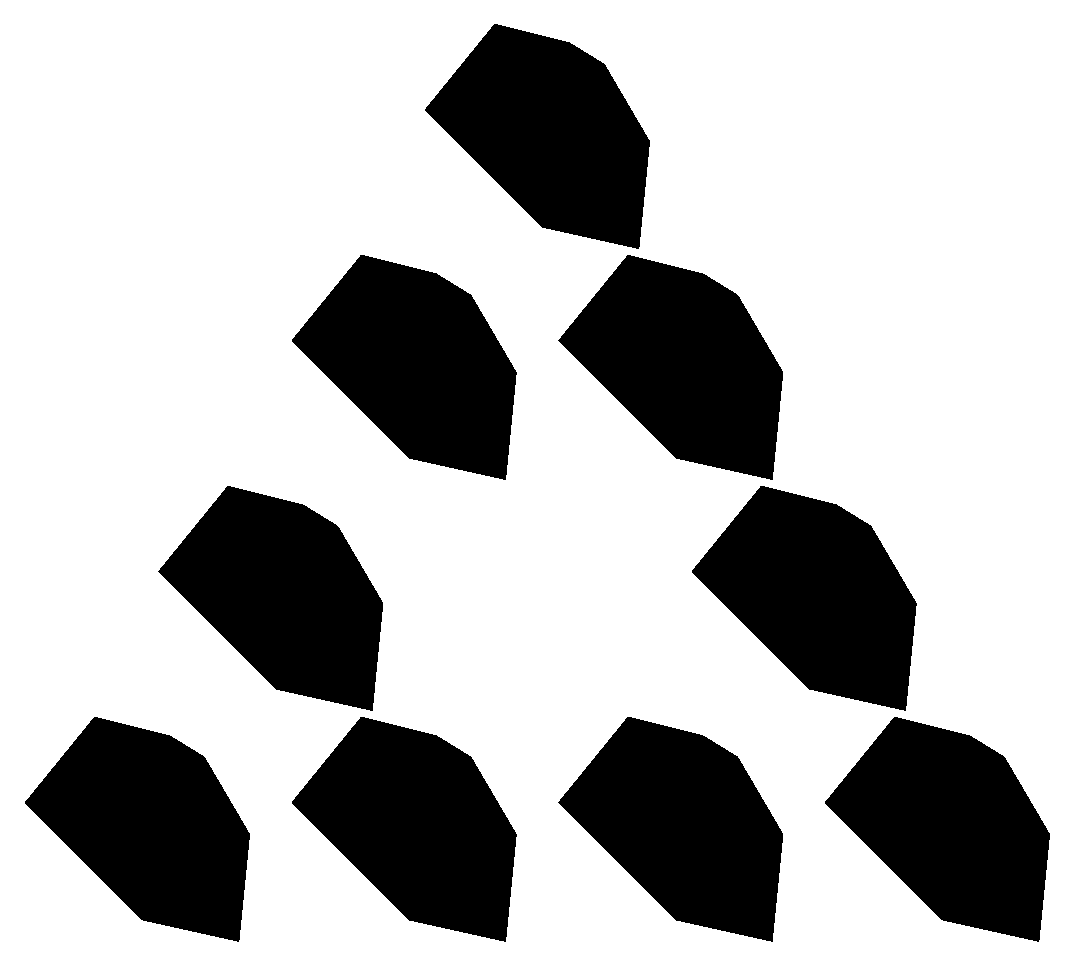
\includegraphics[width=\textwidth]{sierpinsky-triangle-2-iter2.pdf}
        \begin{center}
            $n=2$
        \end{center}
    \end{subfigure}
    \qquad
    \vspace{1cm}
    \begin{subfigure}{0.45\textwidth}
        \centering
        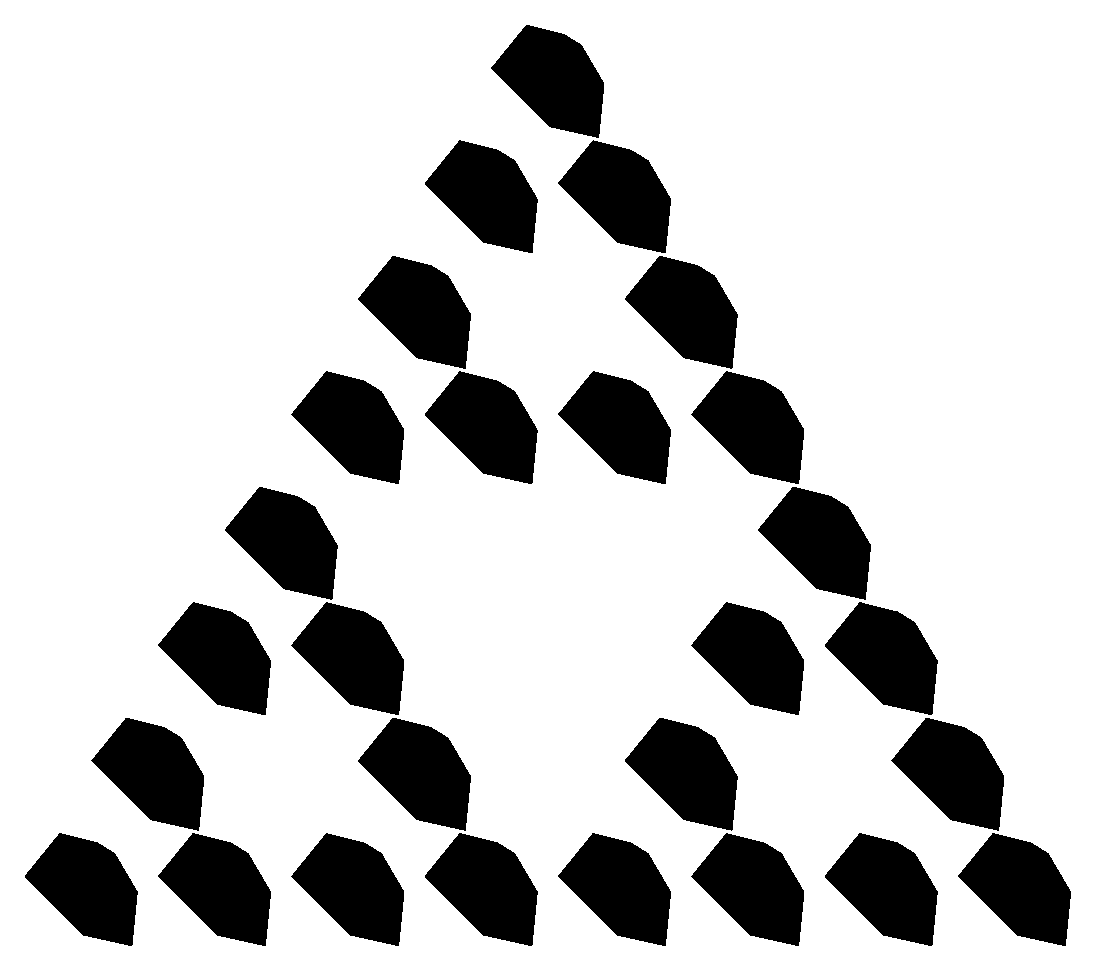
\includegraphics[width=\textwidth]{sierpinsky-triangle-2-iter3.pdf}
        \begin{center}
            $n=3$
        \end{center}
    \end{subfigure}
    \qquad
    \begin{subfigure}{0.45\textwidth}
        \centering
        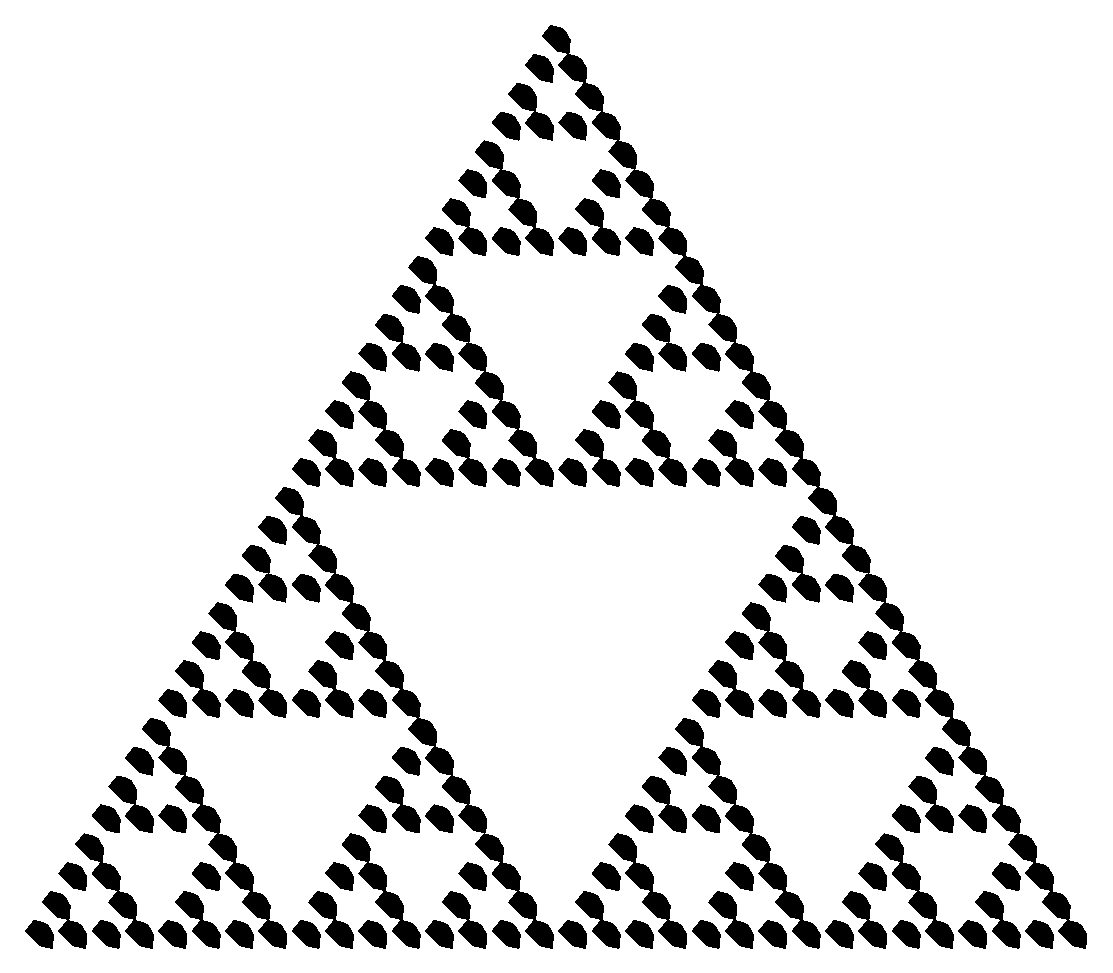
\includegraphics[width=\textwidth]{sierpinsky-triangle-2-iter5.pdf}
        \begin{center}
            $n=5$
        \end{center}
    \end{subfigure}
    \qquad
    \begin{subfigure}{0.45\textwidth}
        \centering
        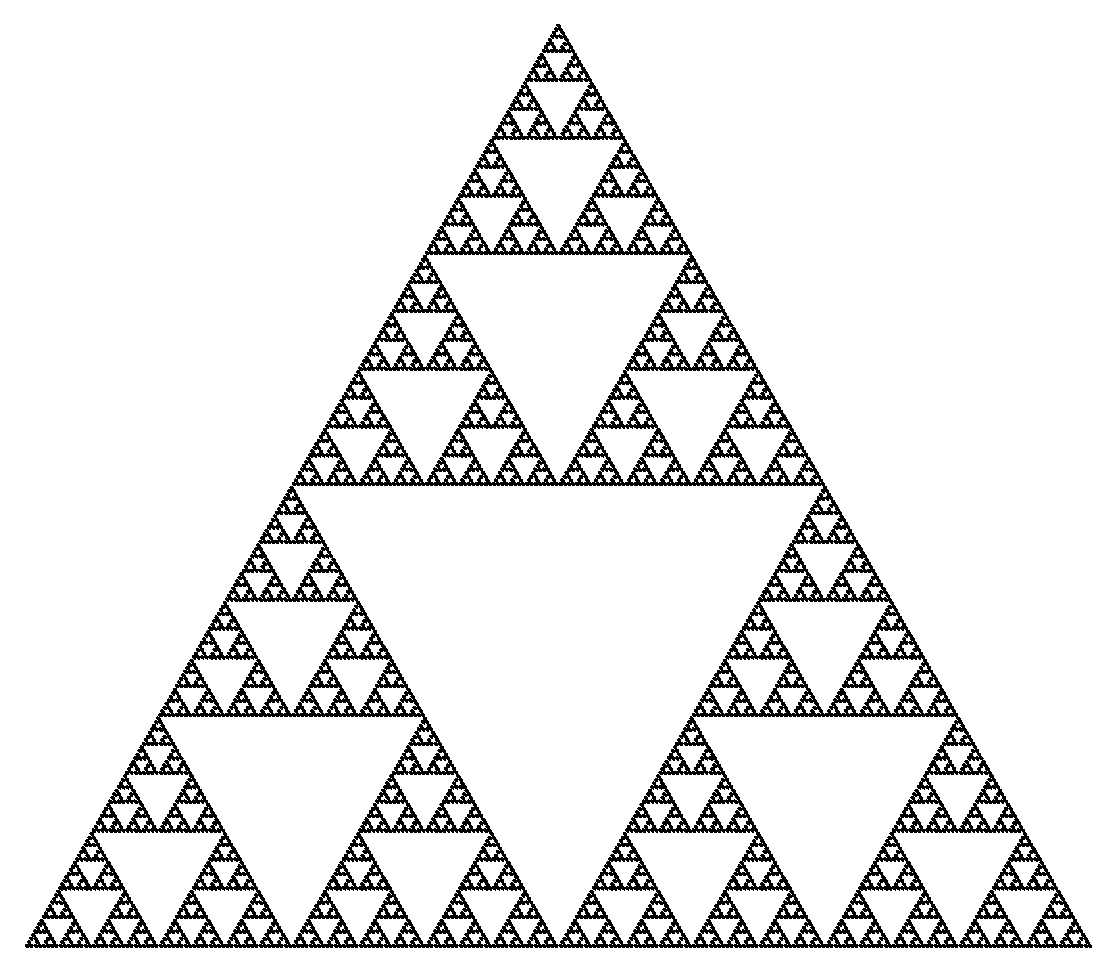
\includegraphics[width=\textwidth]{sierpinsky-triangle-2-iter8.pdf}
        \begin{center}
            $n=8$
        \end{center}
    \end{subfigure}
    \caption{Iterace zobrazení $\Omega$ s jiným počátečním útvarem $B$.}
    \label{fig:iterace-zobrazeni-omega-sierpinskeho-trojuhelnik-jiny-poc-utvar}
\end{figure}
Vypisovat explicitně dané kontrakce je sice formálně žádoucí, nicméně dosti nepraktické. Dále tedy budeme hodnoty jednotlivých koeficientů $a,b,\ldots,f$ (viz \eqref{eq:afinita-v-R2}) zapisovat do tabulky.